\documentclass[10pt,pdf,hyperref={unicode},aspectratio=169]{beamer}

\usepackage{amssymb,amsmath,amsfonts}
\usepackage[T2A]{fontenc}
\usepackage[utf8]{inputenc}
\usepackage[english,russian]{babel}
\usepackage{graphicx}
\usepackage{epstopdf}

\let\chapter\section
\sloppy



\usepackage{amsthm}
\theoremstyle{definition}
\newtheorem{llemma}{Лемма}
\newtheorem{ttheorem}[llemma]{Теорема}
\newtheorem{eexample}[llemma]{Пример}
\newtheorem{property}[llemma]{Свойство}
\newtheorem{remark}[llemma]{Замечание}
\newtheorem{ddefinition}[llemma]{Определение}
\newtheorem{ccorollary}{Следствие}[llemma]



\begin{document}


\title{
	Примеры множеств точек\\с целочисленными расстояниями,\\найденные на ЭВМ
}
\author{Р.Е.~Зволинский, Н.Н.~Авдеев, Е.А.~Момот, А.Е.~Зволинский}
\institute{ Воронежский Государственный Университет \\
		{Работа выполнена  при поддержке РНФ, грант 19-11-00197.
	}}
\date{Воронеж 2021}

\maketitle

\setbeamertemplate{footline}[frame number]
\setbeamertemplate{navigation symbols}{\large{}}


	%%%%%%%%%%%%%%%%%%%%%%%%%%%%%%%%%%%%%%%%%%%%%%%%%%%%%%%%%%%%%%%%%%%%%%%%%%%%%%%%%%%%%%%%%%%

\begin{frame}

	\begin{ddefinition}
		Множеством $\mathcal P$ точек на плоскости с целочисленными расстояниями (сокращённо МЦР) называют
		такое множество не лежащих на одной прямой точек, что расстояние между любыми двумя точками
		из $\mathcal P$ есть целое число.
	\end{ddefinition}

	\vfill

	Всякое МЦР конечно~\cite{bib:01, bib:02} и, следовательно, имеет конечный диаметр
	\begin{equation*}
	    \operatorname{diam} (\mathcal P) = \max_{P_1, P_2 \in \mathcal P}
	    |P_1 P_2|,
	\end{equation*}
	где $|P_1 P_2|$ есть обычное расстояние между точками.

	\vfill

	$\operatorname{char} M = p \quad \Leftrightarrow \quad S_{\triangle ABC} \in \mathbb{Q}\sqrt{p}, ~~ \{A,B,C\}\subset M$

	\vfill
	Пример: характеристика треугольника со сторонами $(1,1,1)$ равна $3$.

\end{frame}

\begin{frame}
	\begin{ddefinition}
		\emph{Веерными (facher)}%
		\footnote{
			По типично европейской традиции, заложенной С. Курцем, классам МЦР даются оригинальные названия;
			например, в~\cite{crabs} изучаются МЦР классов {\it crab} и даже {\it semi-crab}
		}
		называют МЦР мощности $n$, для которых можно найти
		такую прямую $\ell_1$, что $(n - 1)$ точек лежит на $\ell_1$.
	\end{ddefinition}

	\vfill

	Веерные множества встречаются чаще остальных,
	и вопрос о существовании веерного множества с заданными параметрами хорошо изучен в~\cite{bib:04} и \cite[Теорема 5]{bib:05}.

	\vfill

    \begin{figure}[h!]
    	\centering
    	\includegraphics[width=0.7\linewidth]{facher-5.png}
    \end{figure}

\end{frame}

\begin{frame}
	Частичная классификация МЦР введена в~\cite{bib:06}; примеры множеств, в неё не входящих, даны в~\cite{bib:07}.

	\vfill

	Для построения каких-либо общих рассуждений, касающихся существования МЦР некоторого специального вида,
	необходимы наглядные примеры.
	Поиск таких примеров ведётся на ЭВМ и может занимать продолжительное время.
	Авторами разработано ПО на языке NodeJS и опубликовано по адресу gitlab.com/nickkolok/ips-algo
	под свободной лицензией GNU GPLv3.

	\vfill


	Цель данной работы~--- привести примеры МЦР специального вида достаточно большой мощности,
	найденные на ЭВМ.

	\vfill

    \begin{equation*}
        \sqrt p/q * \{(x_1, y_1), \ldots, (x_n, y_n)\} =
        \left\{\left(\frac{x_1}q, \frac{y_1\sqrt p}q\right),
        \ldots, \left(\frac{x_n}q, \frac{y_n\sqrt p}q\right)\right\}.
    \end{equation*}


\end{frame}

\begin{frame}

	\begin{ddefinition}
		\emph{ Ножничными (scissors)} назовём МЦР мощности $n$,
		для которых можно единственным образом найти такие прямые $\ell_1$, $\ell_2$,
		что $k$ точек лежат на $\ell_1$, а $(n - k)$~--- на $\ell_2$, причём $k \geqslant 2$ и
		$\ell_1$ и $\ell_2$ не параллельны и не перпендикулярны.
	\end{ddefinition}


    \begin{figure}[h!]
    	\centering
    	\includegraphics[width=1\linewidth]{25_1544076_91.pdf}
    	%\caption
    	\\~\\{Ножничная МЦР мощности 25, диаметр 1 544 076}
    \end{figure}

    \begin{align*}\footnotesize
        \sqrt{91}/1 * \{ &
		\pm(80784, 12240),
        (0, 0),
        (\pm 772038, 0),
        (\pm 470016, 0),
        \\&
        (\pm 193732, 0),
        (\pm 171564, 0),
        (\pm 126684, 0),
        (\pm 117504, 0),
        \\&
        (\pm 72960, 0),
        (\pm 70686, 0),
        (\pm 65892, 0),
        (\pm 42891, 0),
        (\pm 26112, 0)
        \}
    \end{align*}
\end{frame}

\begin{frame}


    \begin{ddefinition}
		\emph{ Рельсовыми (rails)} называют МЦР
		мощности $n$, для которых можно единственным образом найти такие прямые $\ell_1 \| \ell_2$,
		что $k$ точек лежат на $\ell_1$,
		а $(n - k)$~--- на  $\ell_2$, причём $k \geqslant 2$.
	\end{ddefinition}

	\begin{figure}
		\centering
		\includegraphics[width=1\linewidth]{28_158064_154.pdf}
		\\~\\{Рельсовая МЦР мощности 28, диаметр 158 064}
	\end{figure}

    \begin{align*}
    	\sqrt{154}/1 * \{
		&
    	(\pm 79032, 0),
    	(\pm 49184, 0),
    	(\pm 44352, 0),
    	(\pm 34316, 0),
    	(\pm 33024, 0),
    	(\pm 24864, 0), \\
    	&(\pm 21576, 0),
    	(\pm 20976, -1440),
    	(\pm 20376, 0),
    	(\pm 14712, 0),
    	(\pm 13824, 0),
    	(\pm 8805, 0), \\
    	&(\pm 7232, 0),
    	(\pm 2400, 0)
    	\}
    \end{align*}


\end{frame}

\begin{frame}

    \begin{figure}[h!]
    	\centering
    	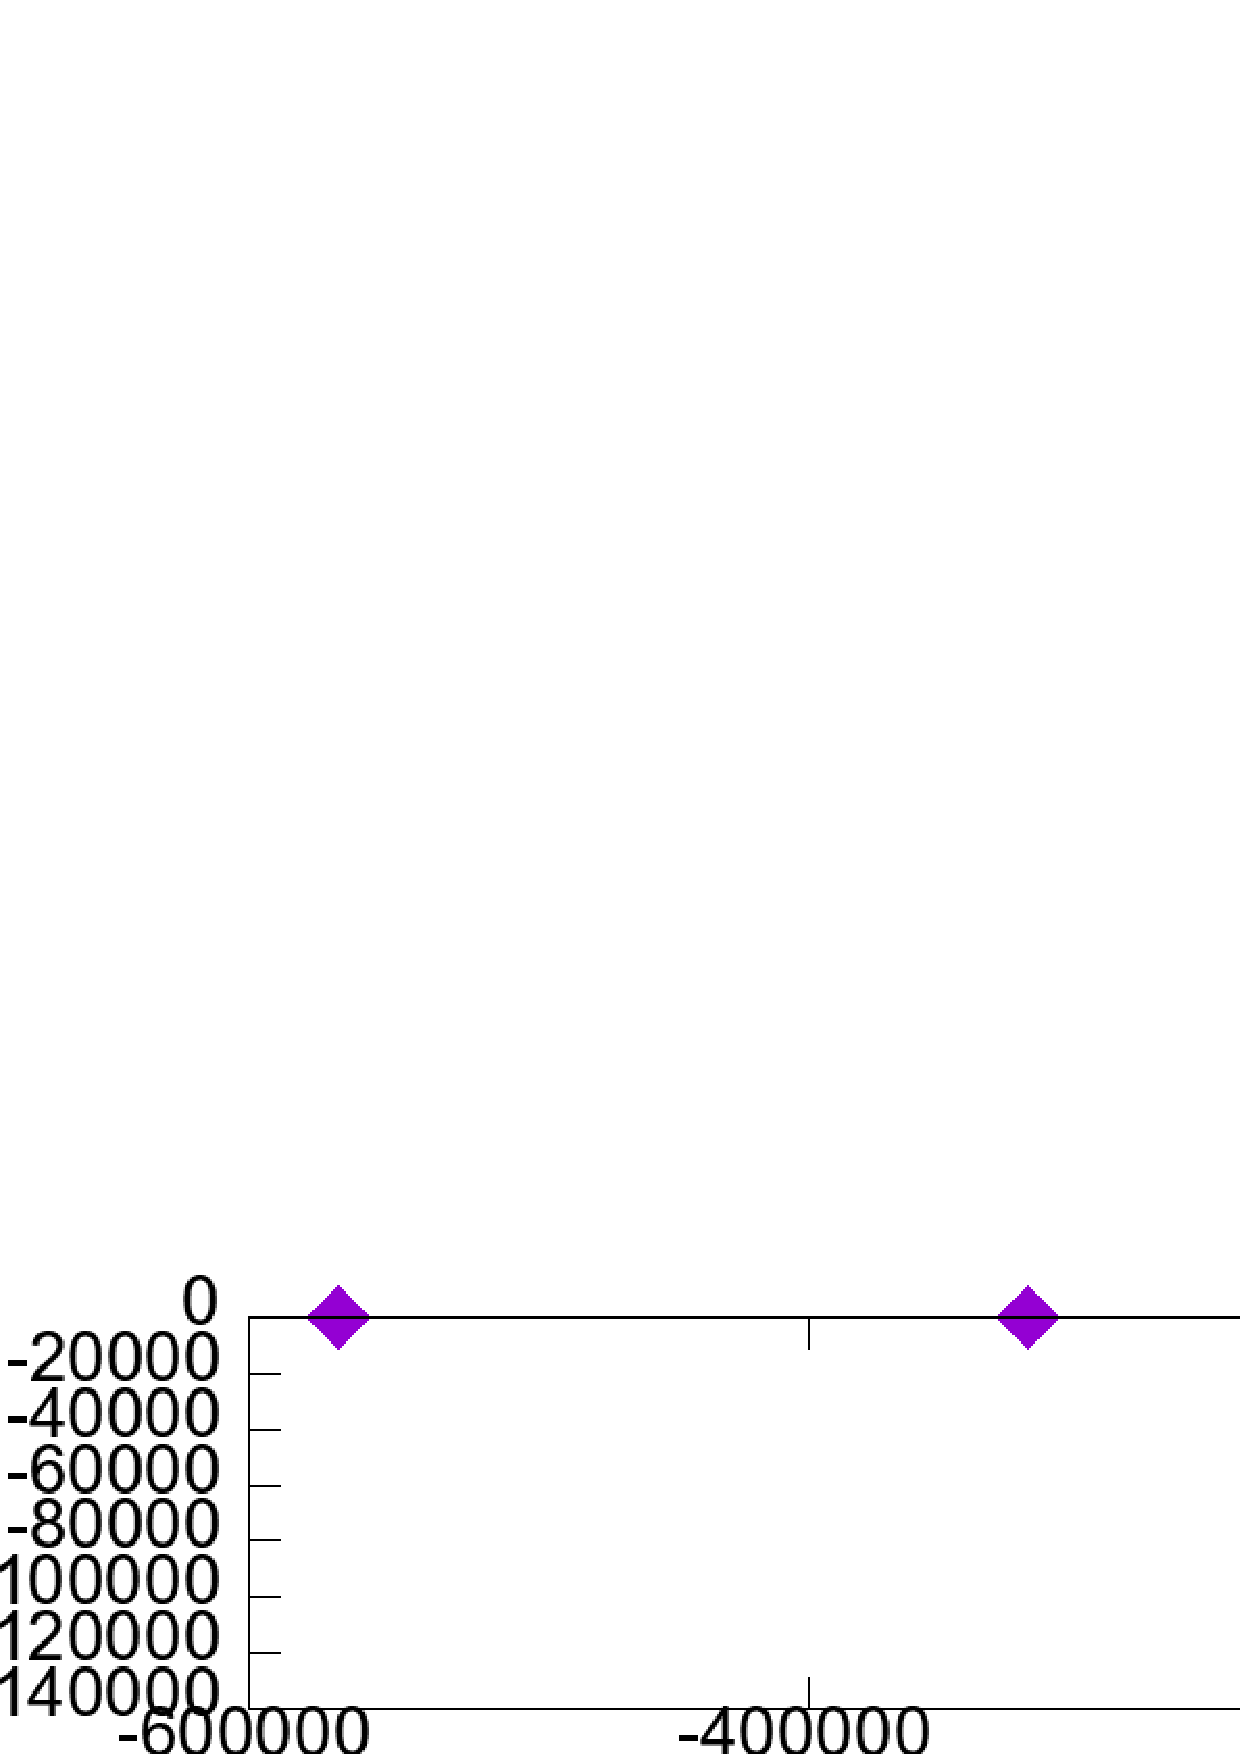
\includegraphics[width=1\linewidth]{32_1598904_154.pdf}
    	\\~\\{Рельсовая МЦР мощности 32, диаметр 1 598 904}
    \end{figure}

    \begin{align*}
    	\sqrt{154}/1 * \{
		&
    	(\pm 799452, 0),
    	(\pm 553224, 0),
    	(\pm 464232, 0),
    	(\pm 344288, 0),
    	(\pm 310464, 0), \\
    	&(\pm 240212, 0),
    	(\pm 231168, 0),
    	(\pm 174048, 0),
    	(\pm 151032, 0),
    	(\pm 146832, -10080), \\
    	&(\pm 142632, 0),
    	(\pm 102984, 0),
    	(\pm 96768, 0),
    	(\pm 61635, 0),
    	(\pm 50624, 0),
    	(\pm 16800, 0)
    	\}
    \end{align*}

\end{frame}

\begin{frame}

    \begin{figure}[h!]
    	\centering
    	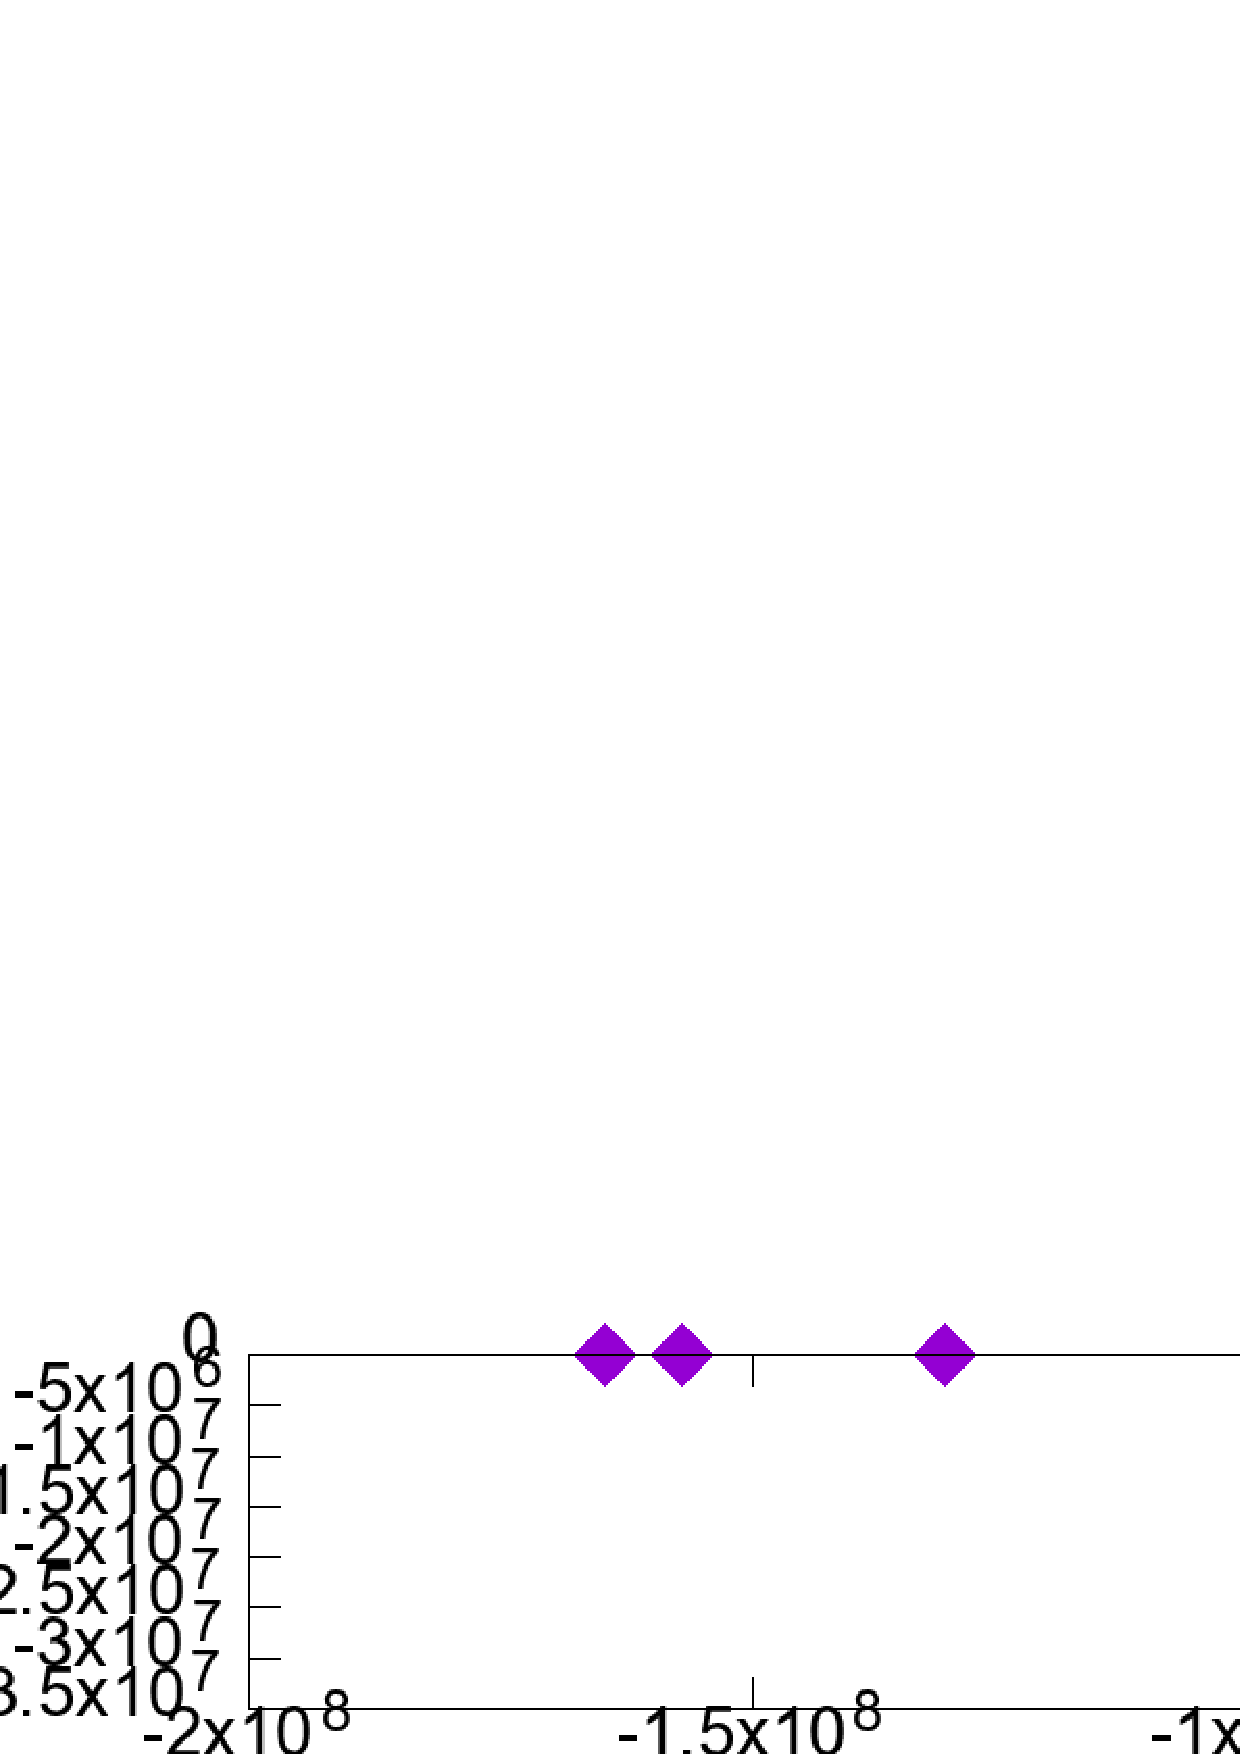
\includegraphics[width=1\linewidth]{44_456989104_154.pdf}
    	\\~\\{Рельсовая МЦР мощности 44, диаметр 456 989 104}
    \end{figure}

    \begin{align*}
    	\sqrt{154}/1 * \{
		&
    	(\pm 228494552, 0),
    	(\pm 220848615, 0),
    	(\pm 194867400, 0),
    	(\pm 152828130, 0), \\
    	&(\pm 128244090, 0),
    	(\pm 95109560, 0),
    	(\pm 85765680, 0),
    	(\pm 66358565, 0),
    	(\pm 63860160, 0), \\
    	&(\pm 62812365, 0),
    	(\pm 48080760, 0),
    	(\pm 41722590, 0),
    	(\pm 40562340, -2784600),
		\\&
    	(\pm 39402090, 0),
    	(\pm 28449330, 0),
    	(\pm 26732160, 0),
    	(\pm 16126320, 0),
    	(\pm 13984880, 0),
		\\&
    	(\pm 8239560, 0),
    	(\pm 4641000, 0),
    	(\pm 3136770, 0),
    	(\pm 2480504, 0)
    	\}
    \end{align*}

\end{frame}

\begin{frame}
    \frametitle{Пример  МЦР, не входящего в существующую классификацию.}

    \begin{figure}[h!]
    	\centering
    	\includegraphics[width=1\linewidth]{23_243663771_1.pdf}
    	\caption{МЦР мощности 23, диаметр 243663771, не входящее в классификацию}
    \end{figure}

    \begin{align*}
    	&\sqrt 1/1 * \{(125570211, 0),
    	(56036760, 0),
    	(44950698, 0),
    	(29275190, 0),
    	(21302190, 0), \\
    	&(\pm 16820310, 0),
    	(12380862, 0),
    	(10722410, 0),
    	(9463662, 0),
    	(8002410, \pm 21162960), \\
    	&(8002410, 0),
    	(4008940, 0),
    	(2627690, 0),
    	(1748940, 0),
    	(-118093560, 0),
    	(-48727185, 0), \\
    	&(-12152790, 0),
    	(-8562390, 0),
    	(-2540310, 0),
    	(-483990, \pm 12252240)
    	\}
    \end{align*}

\end{frame}

\begin{frame}
	Все вычисления "--- с целыми числами \texttt{BigInt}

	\vfill


	Основные проблемы целочисленных вычислений:

	\begin{itemize}
		\item
			Проверка числа на полный квадрат
		\item
			Факторизация
		\item
			Освобождение от квадратов \textit(для вычисления характеристики)
		\item
			Перечисление делителей \textit(для вставки точек)
		\item
			Хранение списков простых чисел
		\item
			Сериализация в JSON
	\end{itemize}

	Опубликованы библиотеки на NPM:

	\begin{itemize}
		\item
			\texttt{bigint-isqrt}
		\item
			\texttt{bigint-is-perfect-square}
		\item
			\texttt{bigint-json-native} \textit(форк)
	\end{itemize}



\end{frame}

\setbeamertemplate{bibliography item}{\insertbiblabel\footnotesize}

\begin{frame}
	\begin{thebibliography}{99}
		\setlength\itemsep{0pt}\scriptsize

		\bibitem{bib:01}
		Anning\,N.\,H., Erd{\"o}s\,P. {\it Integral distances} //~Bulletin of the American Mathematical Society.~--
		1945.~-- Vol.~51.~-- no.~8.~-- С.~598--600.~-- DOI: 10.1090/S0002-9904-1945-08407-9.

		\bibitem{bib:02}
		Erd{\"o}s\,P. {\it Integral distances} //~Bulletin of the American Mathematical Society.~--
		1945.~-- Vol.~51.~-- no.~12.~-- С. 996.~-- DOI: 10.1090/S0002-9904-1945-08490-0.

		\bibitem{crabs}
		Antonov\,A.\,R., Kurz\,S. {\it Maximal integral point sets over $\mathbb{Z}^2$}
		//International Journal of Computer Mathematics.~-- 2010.~-- Т. 87.~-- №. 12.~-- С. 2653-2676.~-- arXiv: 0804.1280[math.CO].

		\bibitem{bib:04}
		Zvolinsky\,R.\,E. {\it Facher integral point sets with particular distances of arbitrary cardinality} //~Актуальные
		проблемы прикладной математики, информатики и механики~-- сб. тр. Междунар. науч. конф.~-- 2020.~-- С.~668--674.

		\bibitem{bib:05}
		Авдеев\,Н.\,Н., Семёнов\,Е.\,М. {\it Множества точек с целочисленными расстояниями на плоскости и в евклидовом пространстве}
		//~Математический форум (Итоги науки. Юг России).~-- 2018.~-- С.~217--236.

		\bibitem{bib:06}
		Avdeev\,N.\,N., Zvolinsky\,R.\,E., Momot\,E.\,A. {\it On particular diameter bounds for integral point sets in higher dimensions.}~--
		2019.~-- arXiv: 1909.10386.

		\bibitem{bib:07}
		Avdeev\,N.\,N., Momot\,E.\,A., Zvolinsky\,A.\,E. {\it On particular examples of planar integral point sets and their classification.}~--
		2021.~-- arXiv: 2102.12462[math.CO].

		\bibitem{bib:08}
		Авдеев\,Н.\,Н. {\it On integral point sets in special position} //~Некоторые вопросы анализа, алгебры, геометрии и
		математического образования: мат-лы междунар. молодежной научной школы <<Актуальные направления математического
		анализа и смежные вопросы>>.~-- 2018.~-- Vol.~8.~-- Pp.~5--6.

		\bibitem{bib:09}
		Авдеев\,Н.\,Н. {\it Об отыскании целоудалённых множеств специального вида}
		//~Актуальные проблемы прикладной математики, информатики и механики~-- сб. тр.
		Международной науч. конф.~-- 2018.~-- С.~492--498.

		\bibitem{bib:03}
		Kemnitz\,A. {\it Punktmengen mit ganzzahligen Abst{\"a}nden.}~-- 1988.
	\end{thebibliography}

\end{frame}

\setbeamertemplate{navigation symbols}{}

\begin{frame}
	{
		\huge\centering
		~\\~\\~\\
		Спасибо за внимание
	}
	~\\
	\vspace{6.28em}
	nickkolok@mail.ru, avdeev@math.vsu.ru
	\\
	github.com/nickkolok
	\\
	gitlab.com/nickkolok
	\\
	arxiv.org/a/avdeev\_n\_1.html
\end{frame}


\end{document}
